%==============================================================================
%  LAB REPORT 4 — DHT11 Sensor Data Reading for Temperature and Humidity
%  Compile with pdfLaTeX (works out of the box on Overleaf).
%
%  >>> PASTE YOUR GOOGLE DRIVE LINKS IN THE MACROS MARKED "EDIT ME" BELOW <<<
%==============================================================================
\documentclass[10pt,a4paper]{article}

%---------------------------------------- page geometry
\usepackage[a4paper,top=2.2cm,bottom=2.0cm,left=2.1cm,right=2.1cm,
            headsep=13pt,footskip=22pt]{geometry}

%---------------------------------------- encoding & fonts
\usepackage[T1]{fontenc}
\usepackage[utf8]{inputenc}
\usepackage{newtxtext,newtxmath}     % Times-like professional text + math
\usepackage[scaled=0.86]{beramono}   % clean monospace for code
\usepackage{microtype}

%---------------------------------------- graphics, colour, boxes
\usepackage{graphicx}
\usepackage[dvipsnames,table]{xcolor}
\usepackage{tikz}
\usepackage{circuitikz}
\usepackage{pgfplots}
\pgfplotsset{compat=1.18}
\usepgfplotslibrary{groupplots}
\usepackage[most]{tcolorbox}
\usepackage{booktabs}
\usepackage{array}
\usepackage{tabularx}
\usepackage{enumitem}
\usepackage{listings}
\usepackage{fancyhdr}
\usepackage{titlesec}
\usepackage{caption}
\usepackage{float}
\usepackage{needspace}
\usetikzlibrary{arrows.meta,positioning,calc,shadows.blur,decorations.pathreplacing}
\ctikzset{bipoles/length=0.62cm}   % compact component symbols

%---------------------------------------- hyperlinks (load late)
\usepackage[hidelinks]{hyperref}
\usepackage{url}
% print a URL stored in a macro, safely (handles _ ~ % etc.)
\newcommand{\showurl}[1]{\expandafter\url\expandafter{#1}}

%==============================================================================
%  Student details
%==============================================================================
\newcommand{\studentname}{Chavan Atharva Sunil}
\newcommand{\rollnumber}{240003021}
\newcommand{\coursecode}{AA303 --- IoT for Space Applications}
\newcommand{\expdate}{10 September 2026}   % <-- CHECK THIS DATE

%  Google Drive folder holding the demonstration videos and the source code
\urldef{\drivefolder}\url{https://drive.google.com/drive/folders/11TP-NX_EF_IpxHlAUYmG8YWPQfst2ae2?usp=sharing}

%==============================================================================
%  Colour palette
%==============================================================================
\definecolor{ink}{HTML}{1B2733}      % body text / headings
\definecolor{accent}{HTML}{0B5FA5}   % primary blue
\definecolor{accentlt}{HTML}{E8F1FA} % pale blue fill
\definecolor{amber}{HTML}{C8791A}    % LED amber
\definecolor{amberlt}{HTML}{FDF3E3}
\definecolor{rule}{HTML}{C9D4DE}
\definecolor{soft}{HTML}{F5F7F9}
\definecolor{codebg}{HTML}{F7F9FB}
\definecolor{cmnt}{HTML}{6C8090}
\definecolor{kw}{HTML}{0B5FA5}
\definecolor{str}{HTML}{1C7C54}
\definecolor{num}{HTML}{9B2D5E}

\color{ink}

%==============================================================================
%  Headings
%==============================================================================
\titleformat{\section}
  {\normalfont\large\bfseries\color{accent}}
  {\raisebox{0pt}{\colorbox{accent}{\color{white}\bfseries\;\thesection\;}}}
  {0.7em}{}[\vspace{2pt}{\color{rule}\titlerule[0.8pt]}]
\titlespacing*{\section}{0pt}{14pt}{8pt}

\titleformat{\subsection}
  {\normalfont\normalsize\bfseries\color{ink}}{\thesubsection}{0.6em}{}
\titlespacing*{\subsection}{0pt}{11pt}{4pt}

\titleformat{\subsubsection}
  {\normalfont\small\bfseries\color{accent}}{}{0em}{}
\titlespacing*{\subsubsection}{0pt}{9pt}{2pt}

%==============================================================================
%  Header / footer
%==============================================================================
\pagestyle{fancy}
\fancyhf{}
\renewcommand{\headrulewidth}{0.4pt}
\renewcommand{\footrulewidth}{0pt}
\fancyhead[L]{\footnotesize\color{cmnt}\textsc{Lab Report 4} \,\textbar\, DHT11 Temperature and Humidity Sensor}
\fancyhead[R]{\footnotesize\color{cmnt}\studentname\ \,\textbar\, \rollnumber}
\fancyfoot[C]{\footnotesize\color{cmnt}\thepage}

%==============================================================================
%  Captions & lists
%==============================================================================
\captionsetup{font=small,labelfont={bf,color=accent},skip=6pt}
\setlist[itemize]{leftmargin=1.35em,itemsep=2pt,topsep=3pt}
\setlist[enumerate]{leftmargin=1.6em,itemsep=2.5pt,topsep=3pt}
\renewcommand{\arraystretch}{1.18}

%==============================================================================
%  Custom boxes
%==============================================================================
\newtcolorbox{keybox}[1][]{
  enhanced, breakable, colback=accentlt, colframe=accent,
  boxrule=0pt, leftrule=3pt, arc=2pt, left=10pt, right=10pt, top=8pt, bottom=8pt,
  fontupper=\normalsize, #1}

\newtcolorbox{notebox}[1][]{
  enhanced, breakable, colback=amberlt, colframe=amber,
  boxrule=0pt, leftrule=3pt, arc=2pt, left=10pt, right=10pt, top=7pt, bottom=7pt,
  fontupper=\small, #1}

\newtcolorbox{titledbox}[2][]{
  enhanced, breakable, colback=white, colframe=rule, boxrule=0.6pt, arc=3pt,
  left=10pt, right=10pt, top=8pt, bottom=8pt,
  title={\bfseries\small #2}, coltitle=white, colbacktitle=accent,
  attach boxed title to top left={xshift=8pt,yshift=-8pt},
  boxed title style={boxrule=0pt,arc=2pt,left=6pt,right=6pt,top=2pt,bottom=2pt},
  #1}

%==============================================================================
%  Code listing style
%==============================================================================
\lstdefinestyle{prostyle}{
  backgroundcolor=\color{codebg},
  basicstyle=\ttfamily\scriptsize\color{ink},
  keywordstyle=\color{kw}\bfseries,
  commentstyle=\color{cmnt}\itshape,
  stringstyle=\color{str},
  numberstyle=\ttfamily\tiny\color{cmnt},
  numbers=left, numbersep=9pt, xleftmargin=17pt, xrightmargin=2pt,
  frame=single, framesep=6pt, rulecolor=\color{rule},
  breaklines=true, showstringspaces=false, tabsize=2,
  columns=fullflexible, keepspaces=true,
  aboveskip=8pt, belowskip=6pt,
  emphstyle=\color{num}\bfseries,
  literate={°}{{$^{\circ}$}}1
}
\lstset{style=prostyle}

%==============================================================================
%  Schematic: Raspberry Pi header -> HW-481 (DHT11) module
%==============================================================================
\newcommand{\dhtschematic}{%
\begin{circuitikz}[scale=0.9, transform shape, every node/.style={font=\footnotesize}]
  % ---- Raspberry Pi header
  \draw[fill=accentlt, draw=accent, line width=0.9pt, rounded corners=4pt]
        (-3.6,-0.35) rectangle (-0.6,3.6);
  \node[text=accent, font=\small\bfseries] at (-2.1,3.1) {Raspberry Pi};
  \node[text=cmnt,   font=\scriptsize]     at (-2.1,2.7) {GPIO header};
  \foreach \y/\pin/\name in {2.0/Pin 1/3.3\,V, 1.1/Pin 3/GPIO2, 0.2/Pin 6/GND}{
     \draw[fill=white, draw=accent, line width=0.6pt] (-0.92,\y-0.14) rectangle (-0.6,\y+0.14);
     \node[anchor=east, font=\scriptsize\bfseries, text=accent, align=right] at (-1.02,\y) {\pin\\[-2pt]{\tiny\color{cmnt}\name}};}
  % ---- wires (colour-coded like the jumper leads used)
  \draw[line width=1.1pt, red!70!black] (-0.6,2.0) -- (3.0,2.0);
  \draw[line width=1.1pt, violet]       (-0.6,1.1) -- (3.0,1.1);
  \draw[line width=1.1pt, black]        (-0.6,0.2) -- (3.0,0.2);
  \node[font=\tiny, text=red!70!black, anchor=south] at (1.2,2.05) {red lead: supply};
  \node[font=\tiny, text=violet,       anchor=south] at (1.2,1.15) {purple lead: data};
  \node[font=\tiny, text=cmnt,         anchor=south] at (1.2,0.25) {black lead: ground};
  % ---- sensor module
  \draw[fill=soft, draw=rule, line width=0.8pt, rounded corners=4pt] (3.0,-0.35) rectangle (7.3,3.6);
  \node[text=ink, font=\small\bfseries] at (5.15,3.15) {HW-481 module};
  \node[text=cmnt, font=\scriptsize] at (5.15,2.78) {DHT11 on a breakout board};
  \foreach \y/\lab in {2.0/$+$, 1.1/S, 0.2/$-$}{
     \draw[fill=white, draw=ink, line width=0.6pt] (3.0,\y-0.14) rectangle (3.32,\y+0.14);
     \node[anchor=west, font=\scriptsize\bfseries] at (3.36,\y) {\lab};}
  % module pull-up between + and S
  \draw[line width=0.7pt] (3.32,2.0) -- (4.4,2.0) to[R, l_=$10\,\mathrm{k}\Omega$] (4.4,1.1) -- (3.32,1.1);
  \node[font=\tiny, text=cmnt, anchor=north] at (4.4,0.95) {pull-up};
  % DHT11 body
  \draw[fill=cyan!20, draw=cyan!60!black, line width=0.8pt] (5.4,0.0) rectangle (7.1,2.5);
  \node[font=\scriptsize\bfseries, text=cyan!40!black, anchor=east] at (7.0,1.25) {DHT11};
  \draw[line width=0.7pt] (4.4,2.0) -- (5.4,2.0); \node[font=\tiny, anchor=west] at (5.42,2.2) {VCC};
  \draw[line width=0.7pt] (4.4,1.1) -- (5.4,1.1); \node[font=\tiny, anchor=west] at (5.42,1.3) {DATA};
  \draw[line width=0.7pt] (3.32,0.2) -- (5.4,0.2); \node[font=\tiny, anchor=west] at (5.42,0.4) {GND};
\end{circuitikz}}

%==============================================================================
\begin{document}

%------------------------------------------------------------------ TITLE BLOCK
\thispagestyle{empty}
\begin{tikzpicture}[remember picture, overlay]
  \fill[accent] (current page.north west) rectangle
        ($(current page.north east)+(0,-7.15cm)$);
  \fill[amber] ($(current page.north west)+(0,-7.15cm)$) rectangle
        ($(current page.north east)+(0,-7.3cm)$);
\end{tikzpicture}

\vspace*{0.35cm}
{\color{white}
 \noindent{\footnotesize\textsc{\coursecode}}\\[2pt]
 \noindent{\Large\bfseries Experiment 4 \,\textbar\, Lab Report}\\[8pt]
 \noindent{\huge\bfseries DHT11 Sensor Data Reading}\\[6pt]
 \noindent{\huge\bfseries for Temperature and Humidity}\\[10pt]
 \noindent{\small Reading a digital temperature and humidity sensor over a single GPIO pin of a Raspberry Pi}
}
\vspace{1.5cm}

\noindent
\begin{tabularx}{\textwidth}{@{}>{\bfseries\color{accent}}l X@{}}
\toprule
Submitted by  & \studentname \\
Roll Number   & \rollnumber \\
Date of Experiment & \expdate \\
Board Used    & Raspberry Pi 4 (BCM numbering, GPIO2 / physical pin 3) \\
\bottomrule
\end{tabularx}

\vspace{10pt}

%------------------------------------------------------------------ 1. AIM
\section{Aim}

\begin{keybox}
To measure \textbf{temperature} and \textbf{relative humidity} with a \textbf{DHT11}
sensor connected to a GPIO pin of a \textbf{Raspberry Pi}. The sensor delivers both
quantities as a digital 40-bit frame over a single data wire; the program on the Pi
requests a reading every two seconds, decodes the frame, checks it, and prints the
temperature in $^{\circ}\mathrm{C}$ and the humidity in \% to the terminal.
\end{keybox}

\subsection*{Objectives}
\begin{itemize}
  \item To connect a DHT11 sensor module to the Raspberry Pi using only three wires ---
        supply, ground and one data line on a GPIO pin.
  \item To understand the sensor's single-wire protocol: the start signal sent by the
        Pi, the sensor's response, and the 40-bit data frame with its checksum.
  \item To read the sensor from Python with the \texttt{adafruit\_dht} library and
        print a continuous stream of temperature and humidity values.
  \item To observe how the readings behave over time, including the occasional failed
        read that the protocol's checksum detects.
\end{itemize}

\subsection*{Brief Theory}
The DHT11 is a low-cost digital sensor that combines a \emph{capacitive humidity
element}, an \emph{NTC thermistor} and a small 8-bit microcontroller in one package.
The microcontroller measures both elements, applies the factory calibration stored in
its memory, and sends the result out as a digital word --- so the host receives
calibrated numbers rather than an analogue voltage that would need an ADC. The sensor
covers $20$--$90\,\%$ relative humidity with an accuracy of $\pm5\,\%$ and
$0$--$50\,^{\circ}\mathrm{C}$ with an accuracy of $\pm2\,^{\circ}\mathrm{C}$, and
it should be polled no faster than once per second (the library used here waits
two seconds between reads).

Communication uses one bidirectional \textbf{single-wire} line, held HIGH by a
pull-up resistor when idle. The host starts a reading by pulling the line LOW for at
least $18\,\mathrm{ms}$ and then releasing it; the sensor answers with an $80\,\mu$s LOW
followed by an $80\,\mu$s HIGH, and then sends \textbf{40 bits}. Every bit begins with
a $50\,\mu$s LOW; the length of the HIGH pulse that follows encodes the value --- about
$26$--$28\,\mu$s for a \texttt{0} and $70\,\mu$s for a \texttt{1}. The 40 bits are five
bytes:
\[
  \underbrace{\mathrm{RH_{int}}}_{\text{byte 1}}\;
  \underbrace{\mathrm{RH_{dec}}}_{\text{byte 2}}\;
  \underbrace{\mathrm{T_{int}}}_{\text{byte 3}}\;
  \underbrace{\mathrm{T_{dec}}}_{\text{byte 4}}\;
  \underbrace{\mathrm{checksum}}_{\text{byte 5}},
  \qquad
  \mathrm{checksum} = (\mathrm{byte}_1+\mathrm{byte}_2+\mathrm{byte}_3+\mathrm{byte}_4) \bmod 256 .
\]
The host measures the pulse widths, assembles the bytes and verifies the checksum; if
the sum does not match, the frame is discarded and the read is repeated. Because the
timing is in microseconds while the Pi runs a multitasking operating system, a
fraction of reads are always lost this way --- which is exactly what the program's
error messages report.

\begin{figure}[htb]
\centering
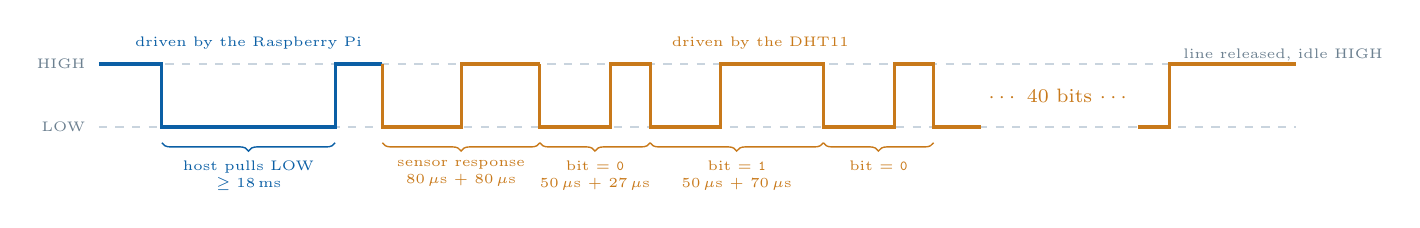
\begin{tikzpicture}[x=1cm, y=0.8cm]
  % baseline levels
  \draw[rule, dashed, line width=0.4pt] (0,0) -- (15.2,0);
  \draw[rule, dashed, line width=0.4pt] (0,1) -- (15.2,1);
  \node[font=\tiny, text=cmnt, anchor=east] at (-0.05,1) {HIGH};
  \node[font=\tiny, text=cmnt, anchor=east] at (-0.05,0) {LOW};
  % host part (accent) : idle high, start low >=18 ms, release
  \draw[accent, line width=1.1pt] (0,1) -- (0.8,1) -- (0.8,0) -- (3.0,0) -- (3.0,1) -- (3.6,1);
  % sensor response (amber): 80 us low, 80 us high
  \draw[amber, line width=1.1pt] (3.6,1) -- (3.6,0) -- (4.6,0) -- (4.6,1) -- (5.6,1);
  % bit 0: 50 us low, 27 us high ; bit 1: 50 us low, 70 us high
  \draw[amber, line width=1.1pt] (5.6,1) -- (5.6,0) -- (6.5,0) -- (6.5,1) -- (7.0,1)
        -- (7.0,0) -- (7.9,0) -- (7.9,1) -- (9.2,1) -- (9.2,0) -- (10.1,0) -- (10.1,1) -- (10.6,1) -- (10.6,0) -- (11.2,0);
  \node[font=\scriptsize, text=amber] at (12.2,0.5) {$\cdots$ 40 bits $\cdots$};
  \draw[amber, line width=1.1pt] (13.2,0) -- (13.6,0) -- (13.6,1) -- (15.2,1);
  % braces / labels
  \draw[decorate, decoration={brace, amplitude=3pt, mirror}, accent, line width=0.5pt]
        (0.8,-0.25) -- (3.0,-0.25) node[midway, below=3pt, font=\tiny, text=accent, align=center] {host pulls LOW\\$\geq 18$\,ms};
  \draw[decorate, decoration={brace, amplitude=3pt, mirror}, amber, line width=0.5pt]
        (3.6,-0.25) -- (5.6,-0.25) node[midway, below=3pt, font=\tiny, text=amber, align=center] {sensor response\\80\,$\mu$s + 80\,$\mu$s};
  \draw[decorate, decoration={brace, amplitude=3pt, mirror}, amber, line width=0.5pt]
        (5.6,-0.25) -- (7.0,-0.25) node[midway, below=3pt, font=\tiny, text=amber, align=center] {bit = \texttt{0}\\50\,$\mu$s + 27\,$\mu$s};
  \draw[decorate, decoration={brace, amplitude=3pt, mirror}, amber, line width=0.5pt]
        (7.0,-0.25) -- (9.2,-0.25) node[midway, below=3pt, font=\tiny, text=amber, align=center] {bit = \texttt{1}\\50\,$\mu$s + 70\,$\mu$s};
  \draw[decorate, decoration={brace, amplitude=3pt, mirror}, amber, line width=0.5pt]
        (9.2,-0.25) -- (10.6,-0.25) node[midway, below=3pt, font=\tiny, text=amber, align=center] {bit = \texttt{0}};
  \node[font=\tiny, text=accent, anchor=south] at (1.9,1.08) {driven by the Raspberry Pi};
  \node[font=\tiny, text=amber,  anchor=south] at (8.4,1.08) {driven by the DHT11};
  \node[font=\tiny, text=cmnt, anchor=west] at (13.65,1.15) {line released, idle HIGH};
\end{tikzpicture}
\caption{The DHT11 single-wire protocol (not to scale). The Pi sends the start
signal; the sensor answers and then clocks out 40 bits, each distinguished by the
width of its HIGH pulse. The last byte is a checksum of the other four.}
\label{fig:protocol}
\end{figure}

\begin{notebox}
\textbf{Note on the module used.} The sensor came as a three-pin \textbf{HW-481}
breakout module, which carries the DHT11 together with its $10\,\mathrm{k}\Omega$ pull-up
resistor on the data line, so no external resistor was needed. The data pin was
connected to \textbf{GPIO2} (physical pin~3). This pin doubles as the I$^2$C SDA line,
so the I$^2$C interface must be disabled in \texttt{raspi-config} for the pin to be free
as a GPIO; it also carries the Pi's own fixed $1.8\,\mathrm{k}\Omega$ pull-up to
$3.3\,\mathrm{V}$, which the DHT11 tolerates.
\end{notebox}

%------------------------------------------------------------------ 2. MATERIALS
\Needspace{8\baselineskip}
\section{Materials Required}

\noindent
\begin{tabularx}{\textwidth}{@{}p{0.4cm} >{\raggedright\arraybackslash}p{5.6cm} c X@{}}
\toprule
\rowcolor{soft}
\multicolumn{1}{@{}l}{\textbf{\#}} & \textbf{Component} & \textbf{Qty.} & \textbf{Purpose in the setup} \\
\midrule
1 & Raspberry Pi 4 (in case, with SD card, OS installed) & 1 & Host board; drives the single-wire bus and runs the program \\
2 & DHT11 sensor module, HW-481 (3-pin, with pull-up)  & 1 & Measures temperature and relative humidity \\
3 & Female--female jumper wires                           & 3 & Supply, data and ground between the header and the module \\
4 & USB-C power supply                                    & 1 & Powering the Raspberry Pi \\
5 & Monitor, keyboard and mouse                           & 1 & Running the program and reading the terminal \\
6 & Software: Python 3, \texttt{adafruit-circuitpython-dht}, \texttt{libgpiod2} & --- & Library that implements the DHT11 protocol \\
\bottomrule
\end{tabularx}

%------------------------------------------------------------------ 3. METHODOLOGY
\section{Methodology}

No breadboard was needed: the module's three pins were connected straight to the
Raspberry Pi's header with three jumper wires --- supply to the $3.3\,\mathrm{V}$ pin,
ground to a GND pin, and the signal pin to GPIO2. The Adafruit DHT library was
installed, and a short Python program was written that creates a \texttt{DHT11} object
on \texttt{board.D2}, then loops forever reading \texttt{temperature} and
\texttt{humidity} from it every two seconds and printing them. Failed reads --- which
the library reports as a \texttt{RuntimeError} when the checksum does not match or the
frame is incomplete --- are caught, printed, and simply retried on the next cycle.

\subsection{Connections}

\vspace{2pt}
\noindent
\begin{minipage}[t]{0.5\textwidth}
\vspace{0pt}
\begin{tabularx}{\linewidth}{@{}l l >{\raggedright\arraybackslash}X@{}}
\toprule
\rowcolor{soft}
\textbf{Module pin} & \textbf{Raspberry Pi} & \textbf{Jumper} \\
\midrule
$+$ (VCC)    & Pin 1 --- $3.3\,\mathrm{V}$     & red \\
S (signal)   & Pin 3 --- GPIO2 (\texttt{board.D2}) & purple \\
$-$ (GND)    & Pin 6 --- GND                   & black \\
\bottomrule
\end{tabularx}
\end{minipage}\hfill
\begin{minipage}[t]{0.47\textwidth}
\vspace{0pt}
\begin{titledbox}[unbreakable]{Numbering used here}
\raggedright
The \texttt{board} module of CircuitPython names pins by their \textbf{BCM} GPIO number,
so \texttt{board.D2} is GPIO2, which sits at \emph{physical} pin~3 of the 40-pin header
--- the second pin on the inner row, right next to the $3.3\,\mathrm{V}$ pin used for
the supply. The three connections therefore all fall within the first three rows of
the header.
\end{titledbox}
\end{minipage}

\begin{figure}[htb]
\centering
\dhtschematic
\caption{Circuit schematic. The HW-481 module needs only supply, ground and one data
line; its on-board $10\,\mathrm{k}\Omega$ resistor holds the data line HIGH when neither
side is driving it.}
\label{fig:schematic}
\end{figure}

\Needspace{12\baselineskip}
\subsection{Software setup}

The \texttt{adafruit\_dht} library implements the microsecond-level protocol of
Figure~\ref{fig:protocol} in native code, so the Python program only has to ask for a
value. It was installed on Raspberry Pi OS with:

\begin{lstlisting}[language=bash, caption={Installing the DHT library on Raspberry Pi OS.}, label={lst:install}]
sudo apt install libgpiod2
pip3 install adafruit-circuitpython-dht
\end{lstlisting}

\noindent The library depends on Adafruit \emph{Blinka}, which provides the
\texttt{board} module that maps names such as \texttt{D2} to the Pi's GPIO pins.

\subsection{Procedure}
\begin{enumerate}
  \item With the Raspberry Pi powered off, the module's $+$, S and $-$ pins were
        connected with three jumper wires to pin~1 ($3.3\,\mathrm{V}$), pin~3 (GPIO2) and
        pin~6 (GND) of the header, and the connections were checked against the pinout.
  \item The Pi was booted, the I$^2$C interface was confirmed to be disabled, and the
        library of Listing~\ref{lst:install} was installed.
  \item The program of Listing~\ref{lst:dht} was saved as \texttt{dht.py} and started
        from the terminal with \texttt{python3 dht.py}.
  \item The terminal was observed while the program printed a new temperature and
        humidity pair every two seconds; the readings were recorded on video, together
        with the error lines produced whenever a frame failed its checksum.
  \item The program was stopped with \texttt{Ctrl+C}, which releases the sensor and
        the GPIO pin.
\end{enumerate}

\Needspace{24\baselineskip}
\subsection{Code (Python, Raspberry Pi)}

\begin{lstlisting}[language=Python, caption={Reading the DHT11 every two seconds and printing temperature and humidity.}, label={lst:dht}]
import time
import board
import adafruit_dht

# HW-481 (DHT11) signal pin connected to GPIO2 = physical pin 3
dht = adafruit_dht.DHT11(board.D2)

try:
    while True:
        try:
            temperature = dht.temperature      # degrees Celsius
            humidity = dht.humidity            # percent relative humidity
            print(f"Temperature: {temperature:.1f} °C")
            print(f"Humidity:    {humidity:.1f} %")
            print("-" * 28)
        except RuntimeError as error:
            # A failed frame (bad checksum, incomplete data) is normal for
            # a DHT sensor on a non-real-time OS: report it and try again.
            print("DHT reading error:", error.args[0])
        time.sleep(2.0)                        # DHT11 needs >= 1 s between reads

except KeyboardInterrupt:
    print("\nExiting program")

finally:
    dht.exit()                                 # release the pin and the sensor
\end{lstlisting}

%------------------------------------------------------------------ 4. RESULT
\Needspace{16\baselineskip}
\section{Result and Output}

\begin{keybox}
The sensor was read successfully over the single data wire. The program printed a
temperature and humidity pair every two seconds; over the recorded run of
\textbf{18 readings} the temperature fell steadily from $30.9$ to
$28.7\,^{\circ}\mathrm{C}$ while the relative humidity rose from $46$ to $53\,\%$.
Four attempts in the same run failed the checksum or returned an incomplete frame;
each was reported by the program and the next read succeeded.
\end{keybox}

\subsection*{Observed outputs}

\vspace{2pt}
\noindent
\begin{minipage}[t]{0.48\textwidth}
\vspace{0pt}
\begin{tabularx}{\linewidth}{@{}c c c X@{}}
\toprule
\rowcolor{soft}
\textbf{\#} & \textbf{Temp.\ ($^{\circ}$C)} & \textbf{RH (\%)} & \textbf{Remark} \\
\midrule
1 & 30.9 & 46 & \\
2 & 30.9 & 46 & \\
3 & 30.8 & 47 & \\
4 & 30.6 & 47 & \\
5 & 30.5 & 47 & \\
6 & 30.3 & 48 & \\
7 & 30.2 & 48 & \\
8 & 30.1 & 48 & then 2 checksum errors \\
9 & 29.8 & 49 & then 1 incomplete frame \\
\bottomrule
\end{tabularx}
\end{minipage}\hfill
\begin{minipage}[t]{0.48\textwidth}
\vspace{0pt}
\begin{tabularx}{\linewidth}{@{}c c c X@{}}
\toprule
\rowcolor{soft}
\textbf{\#} & \textbf{Temp.\ ($^{\circ}$C)} & \textbf{RH (\%)} & \textbf{Remark} \\
\midrule
10 & 29.6 & 50 & \\
11 & 29.4 & 50 & then 1 checksum error \\
12 & 29.3 & 51 & \\
13 & 29.1 & 51 & \\
14 & 29.1 & 51 & \\
15 & 29.0 & 52 & \\
16 & 28.8 & 52 & \\
17 & 28.8 & 52 & \\
18 & 28.7 & 53 & \\
\bottomrule
\end{tabularx}
\end{minipage}

\vspace{8pt}
\noindent The 18 values were transcribed from the terminal as recorded in the two video
clips, which are consecutive (the last reading visible in the first clip is the first
in the second). With the program's two-second interval the run spans roughly
$45\,\mathrm{s}$ including the four failed attempts.

\begin{figure}[H]
\centering
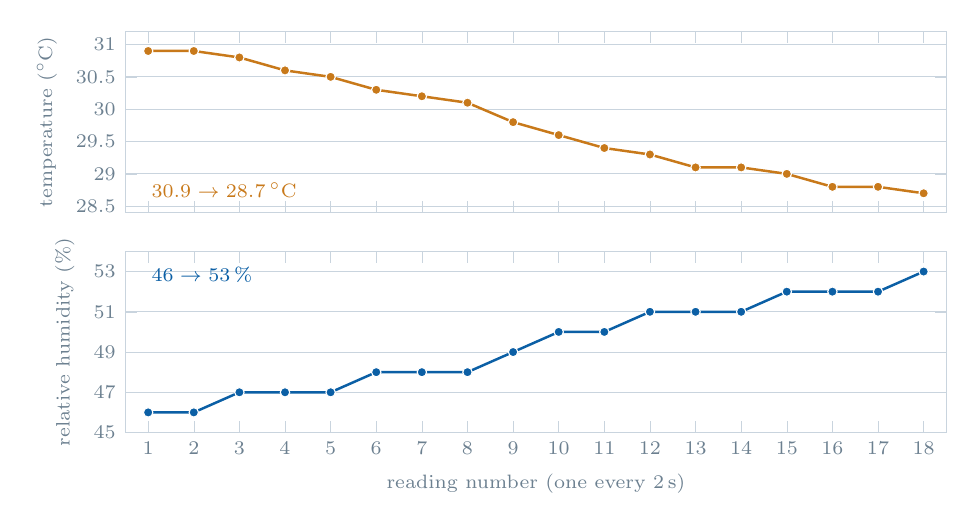
\begin{tikzpicture}
\begin{groupplot}[
  group style={group size=1 by 2, vertical sep=14pt, x descriptions at=edge bottom},
  width=0.86\textwidth, height=2.3cm, scale only axis,
  xmin=0.5, xmax=18.5, xtick={1,2,...,18},
  tick label style={font=\scriptsize, color=cmnt},
  axis line style={rule, line width=0.4pt}, tick style={rule},
  ymajorgrids, grid style={rule, line width=0.3pt},
  ylabel style={font=\scriptsize, color=cmnt},
  xlabel={reading number (one every 2\,s)}, xlabel style={font=\scriptsize, color=cmnt},
  clip=false]
\nextgroupplot[ymin=28.4, ymax=31.2, ytick={28.5,29.0,29.5,30.0,30.5,31.0},
               ylabel={temperature ($^{\circ}$C)}]
\addplot[amber, line width=0.9pt, mark=*, mark size=1.7pt, mark options={fill=amber, draw=white, line width=0.4pt}]
  coordinates {(1,30.9) (2,30.9) (3,30.8) (4,30.6) (5,30.5) (6,30.3) (7,30.2) (8,30.1) (9,29.8)
               (10,29.6) (11,29.4) (12,29.3) (13,29.1) (14,29.1) (15,29.0) (16,28.8) (17,28.8) (18,28.7)};
\node[anchor=south west, font=\scriptsize, text=amber] at (rel axis cs:0.02,0.03) {$30.9 \to 28.7\,^{\circ}$C};
\nextgroupplot[ymin=45, ymax=54, ytick={45,47,49,51,53}, ylabel={relative humidity (\%)}]
\addplot[accent, line width=0.9pt, mark=*, mark size=1.7pt, mark options={fill=accent, draw=white, line width=0.4pt}]
  coordinates {(1,46) (2,46) (3,47) (4,47) (5,47) (6,48) (7,48) (8,48) (9,49)
               (10,50) (11,50) (12,51) (13,51) (14,51) (15,52) (16,52) (17,52) (18,53)};
\node[anchor=north west, font=\scriptsize, text=accent] at (rel axis cs:0.02,0.97) {$46 \to 53\,\%$};
\end{groupplot}
\end{tikzpicture}
\caption{The 18 recorded readings. Temperature (top) drifts down by
$2.2\,^{\circ}\mathrm{C}$ over the run while relative humidity (bottom) climbs by
$7\,\%$ --- the two move in opposite directions, as expected for air whose moisture
content is not changing (see Discussion). The four failed attempts fell between
readings 8--9, 9--10 and 11--12 and do not appear as points.}
\label{fig:trend}
\end{figure}

\subsection*{Recorded outputs --- Raspberry Pi terminal}

\begin{figure}[H]
\centering
\begin{minipage}[t]{0.26\textwidth}
\centering
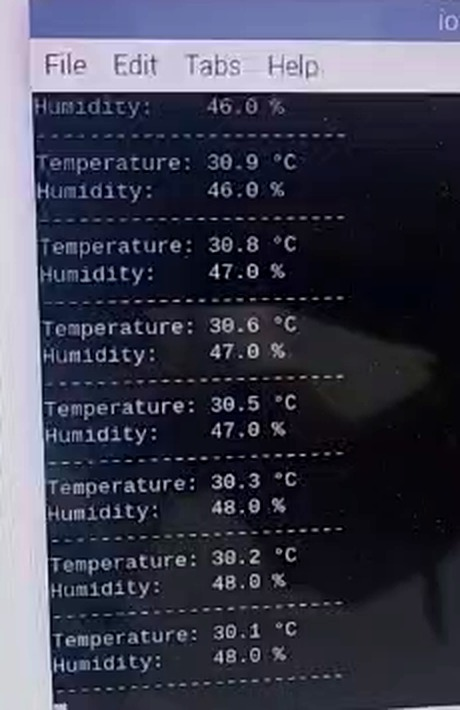
\includegraphics[width=\linewidth]{figures/terminal_1.jpg}\\[2pt]
{\scriptsize\color{cmnt} readings 1--8}
\end{minipage}\hfill
\begin{minipage}[t]{0.355\textwidth}
\centering
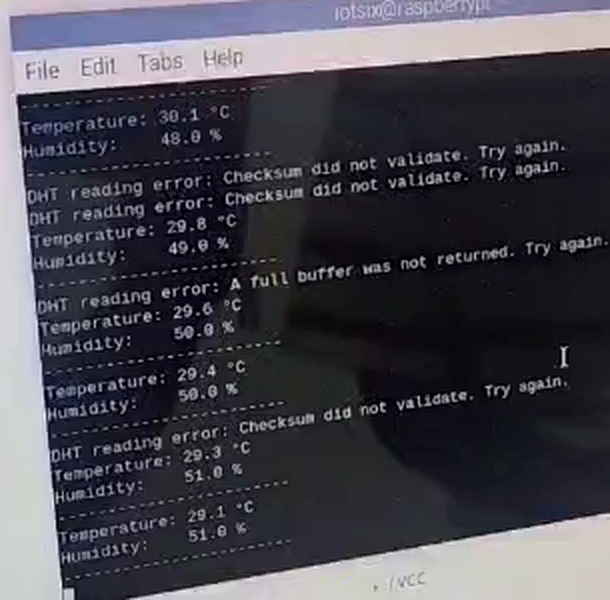
\includegraphics[width=\linewidth]{figures/terminal_2.jpg}\\[2pt]
{\scriptsize\color{cmnt} readings 8--13, with the four failed reads}
\end{minipage}\hfill
\begin{minipage}[t]{0.355\textwidth}
\centering
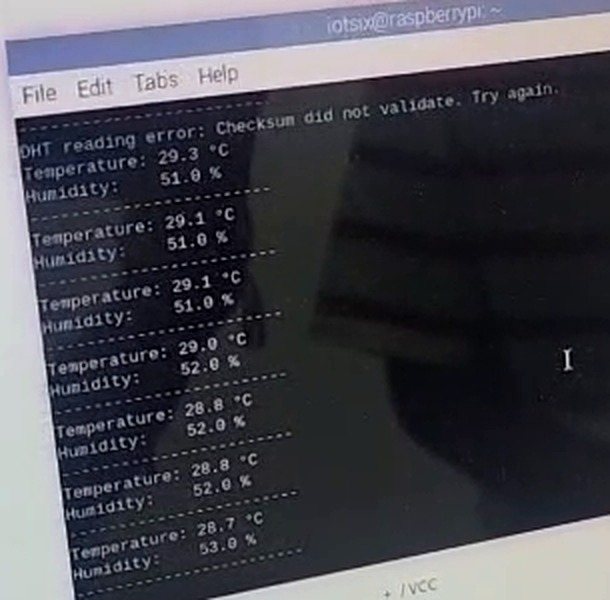
\includegraphics[width=\linewidth]{figures/terminal_3.jpg}\\[2pt]
{\scriptsize\color{cmnt} readings 12--18}
\end{minipage}
\caption{Three frames from the recording of the terminal on the Raspberry Pi while
\texttt{dht.py} was running. Each successful read prints a temperature and a humidity
line followed by a rule; a failed read prints \texttt{DHT reading error:} with the
library's message --- \emph{Checksum did not validate} when the fifth byte does not
match the other four, and \emph{A full buffer was not returned} when fewer than 40
bits were captured.}
\label{fig:terminal}
\end{figure}

\begin{figure}[H]
\centering
\begin{minipage}[t]{0.6\textwidth}
\vspace{0pt}
\centering
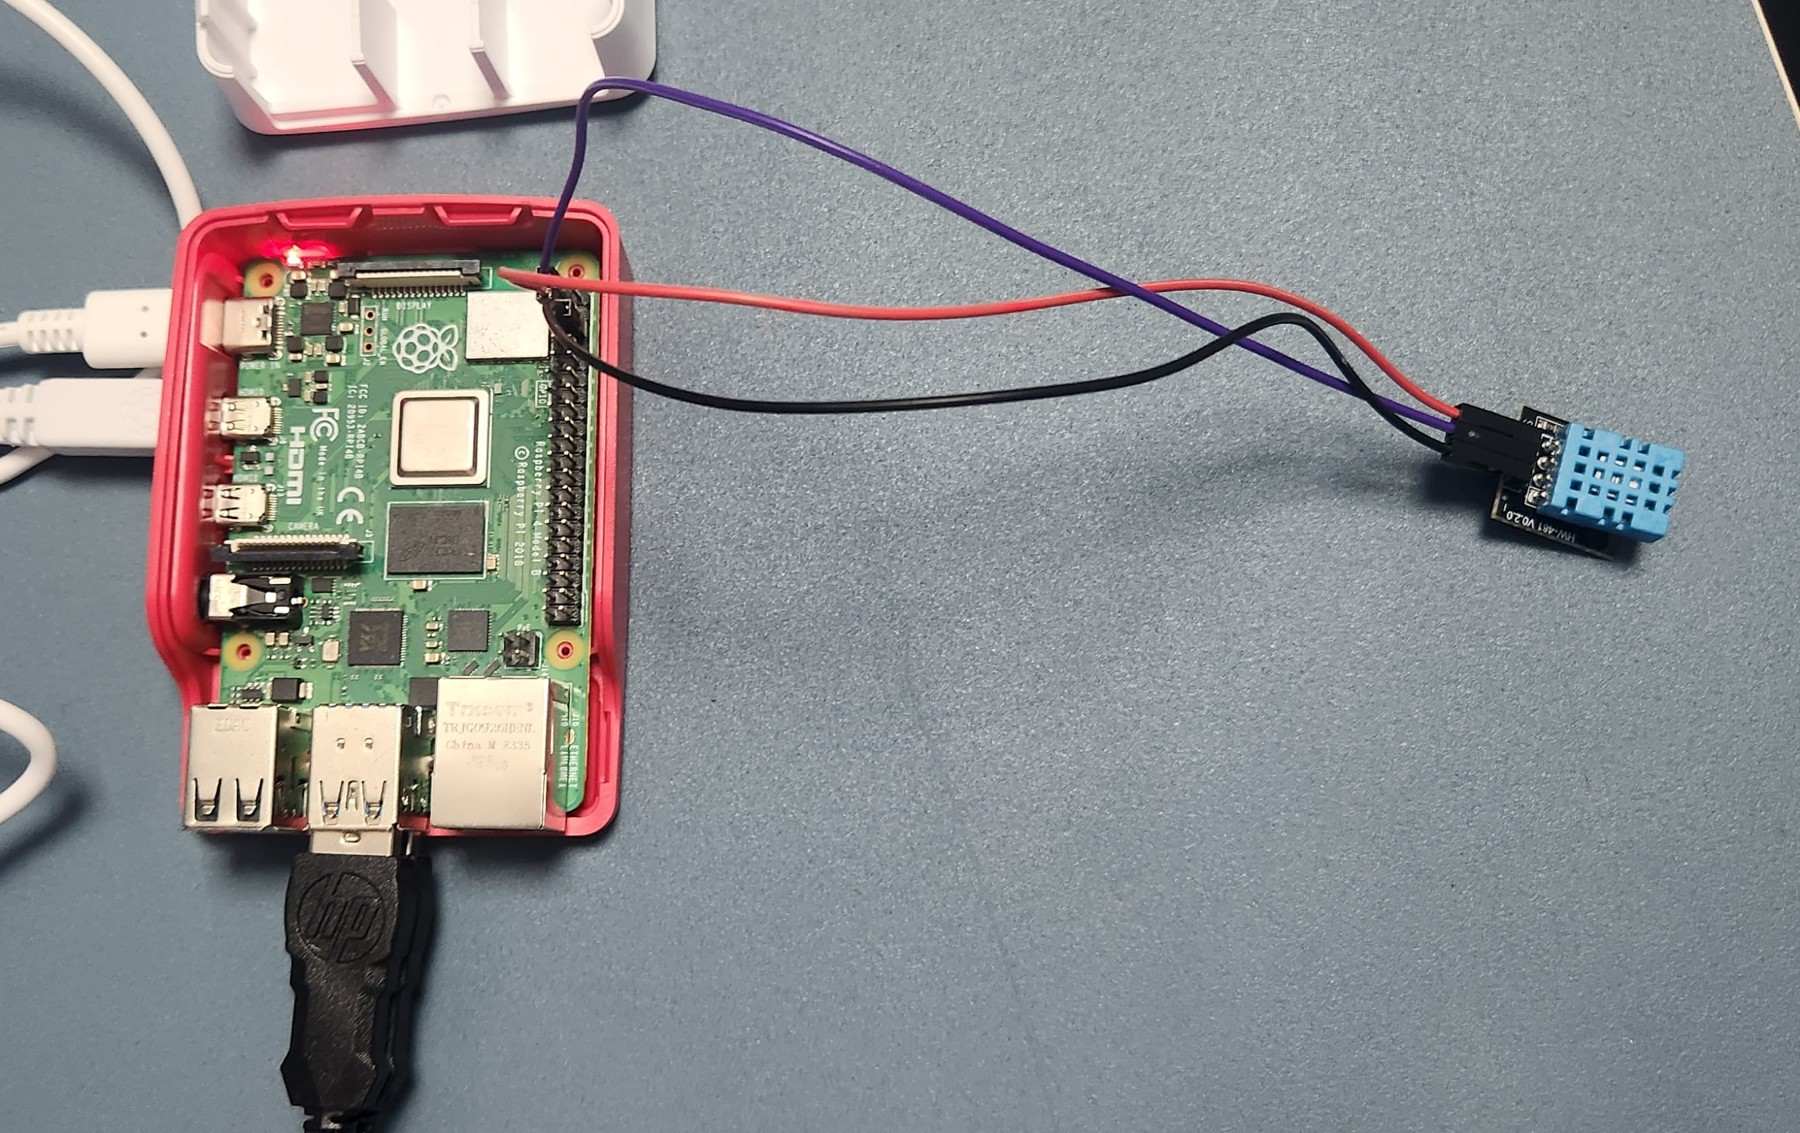
\includegraphics[width=\linewidth]{figures/dht11_setup.jpg}
\end{minipage}\hfill
\begin{minipage}[t]{0.37\textwidth}
\vspace{0pt}
\centering
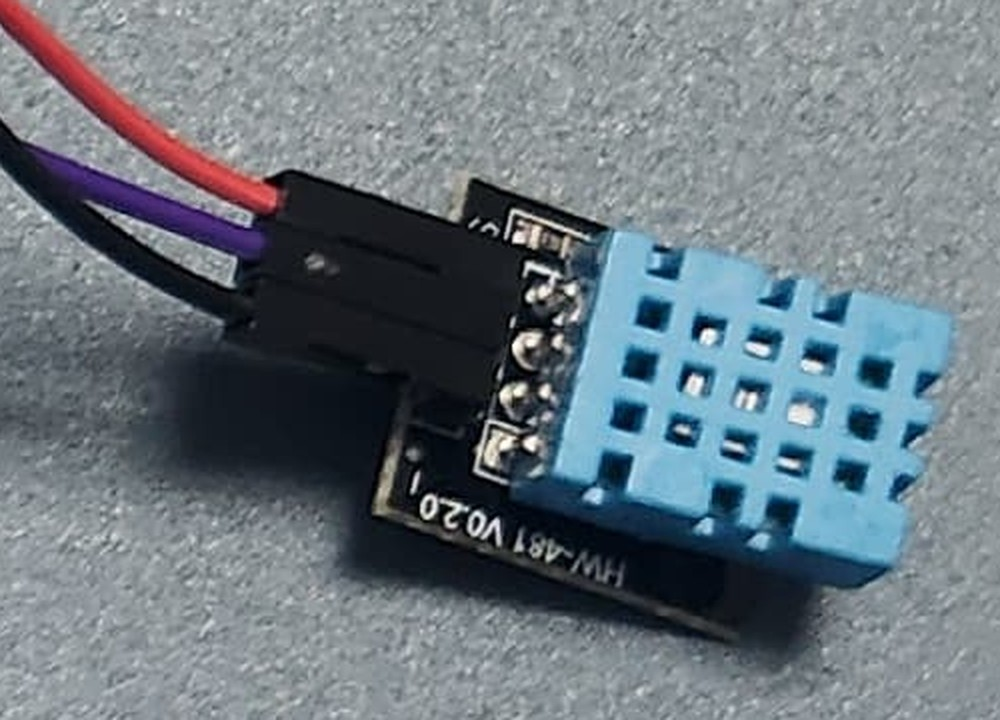
\includegraphics[width=\linewidth]{figures/dht11_module.jpg}
\end{minipage}
\caption{\emph{Left:} the Raspberry Pi 4 with the DHT11 module hanging off three jumper
wires --- red to $3.3\,\mathrm{V}$, purple to GPIO2, black to GND --- entering the first
rows of the GPIO header. \emph{Right:} the HW-481 module (marked ``HW-481 V0.2.0'')
carrying the blue DHT11 and its pull-up resistor.}
\label{fig:setup}
\end{figure}

\subsection*{Video demonstration and code}

\begin{titledbox}[before skip=6pt]{Google Drive link}
\noindent The demonstration videos, this report and the complete source code are
available in the following shared folder:

\vspace{4pt}
\noindent\drivefolder

\vspace{4pt}
{\small\color{cmnt} Access has been set to \emph{anyone with the link can view}.}
\end{titledbox}

\subsection*{Discussion}
\label{sec:discussion}
\begin{itemize}
  \item \textbf{Why the readings drift.} The temperature fell by
        $2.2\,^{\circ}\mathrm{C}$ and the humidity rose by $7\,\%$ over less than a
        minute. The sensor had just been handled while wiring it, so it started warmer
        than the room air and cooled towards it. Relative humidity is the ratio of the
        water vapour present to the maximum the air can hold at that temperature, and
        the maximum falls as the air cools; with the same moisture content, RH
        therefore rises as the temperature drops --- exactly the opposite-going curves
        of Figure~\ref{fig:trend}.
  \item \textbf{Failed reads are expected.} Four of 22 attempts failed. The bit
        timing of the protocol is measured in tens of microseconds, but Raspberry Pi OS
        is not a real-time system and can pre-empt the reading routine at any moment,
        stretching a pulse or losing the end of the frame. The checksum catches the
        corrupted frames, and the correct response is simply to discard them and read
        again --- which the program does by catching the \texttt{RuntimeError}.
  \item \textbf{Resolution and accuracy.} The values are printed to one decimal place
        but the DHT11 is only specified to $\pm2\,^{\circ}\mathrm{C}$ and $\pm5\,\%$
        RH, and the humidity byte here changes only in whole percent. The decimal
        place is useful for seeing the \emph{trend}, not as an absolute accuracy. For
        better figures the pin-compatible DHT22 ($\pm0.5\,^{\circ}\mathrm{C}$,
        $\pm2\,\%$) can be swapped in by changing one line of the program.
  \item \textbf{The single-wire interface.} Unlike the earlier experiments, in which
        the GPIO pin was only ever an output, here the same pin is driven by the Pi for
        the start signal and then switched to an input to listen to the sensor. Two
        pull-ups end up in parallel on the line --- the module's $10\,\mathrm{k}\Omega$
        and the Pi's $1.8\,\mathrm{k}\Omega$ on GPIO2 --- giving about
        $1.5\,\mathrm{k}\Omega$, which the DHT11 can still pull LOW. On a pin without a
        board pull-up (say GPIO4) only the module's resistor would be present.
  \item \textbf{Sampling rate.} The two-second delay is not just politeness: the
        DHT11 needs at least a second between conversions, and reading it faster
        returns stale or invalid data.
\end{itemize}

%------------------------------------------------------------------ CONCLUSION
\Needspace{12\baselineskip}
\section{Conclusion}

The experiment moved from driving outputs to \textbf{acquiring data}: a DHT11 sensor
was read from a single GPIO pin of a Raspberry Pi, returning calibrated temperature
and relative humidity as a checksummed digital frame, and the program printed a fresh
pair of values every two seconds. Eighteen consecutive readings showed the sensor
settling from $30.9$ to $28.7\,^{\circ}\mathrm{C}$ with humidity rising from $46$ to
$53\,\%$, the two quantities moving in opposite directions as the physics of relative
humidity predicts, and the four frames that failed the checksum were detected and
discarded rather than reported as false values.

The exercise showed the practical side of a digital sensor interface --- installing a
driver library, the meaning of its error messages, and the timing limitations of a
general-purpose operating system --- and it produces the kind of environmental data
that an IoT node would log or transmit, which is where the following experiments lead.

\end{document}
